\documentclass[12pt]{article}

\newcommand\tab[1][1cm]{\hspace*{#1}}

\usepackage{times}
\usepackage{amsmath}
\usepackage{latexsym}
\usepackage{fullpage}
\usepackage{graphicx}
\usepackage{amsfonts}
\usepackage[dvipsnames]{xcolor}

\graphicspath{ {./images/} }

\newcommand{\NOT}{\neg}
\newcommand{\AND}{\wedge}
\newcommand{\OR}{\vee}
\newcommand{\XOR}{\oplus}
\newcommand{\IMPLIES}{\rightarrow}
\newcommand{\IFF}{\leftrightarrow}
\newcommand{\E}{\exists}
\newcommand{\A}{\forall}

\setlength{\parskip}{.1in}

\renewcommand{\baselinestretch}{1.1}

\begin{document}

\begin{center}

{\bf
CSCE 313\\
Quiz 2\\
Jeffrey Xu\\
527008162\\
09/18/20\\
}

\end{center}

{\bf 1.} [5 pts] While implementing the process state diagram, what is the problem of having only 1 queue for all blocked processes waiting for all events? What is the solution to this problem? Describe with an example.

The issue of having one queue is that is cannot handle different types of events. If a queue with a bunch of different processes waiting for different I/O events has a process at the front that is waiting for a keyboard interrupt but currently an audio I/O hits, then the queue can't really process the event that is waiting for the audio I/O as it isn't in the front. The queue is essentially a priority queue but with an undefined priority. The only way for having one queue is to have an oracle that can see into the future and assign priorities based on which I/O event will occur first. However, since we do not have the ability to time travel or predict the future with any more accuracy than a man throwing darts at a board while blindfolded, we must think of a more clever solution to our issue. 

The solution to this is to have queues for every single type of I/O. This takes away the "priority" sense of the queue and allows processes to be handled with other similar processes. Now, given our original queue, there is a queue for keyboard interrupt and another separate queue for audio I/O. If there is an audio I/O interrupt, the first element in the audio queue will get popped off and sent to the next state for processing. This allows the blocking mechanism to still work in $O(1)$ without too much overhead while still using the same amount of space. 

{\bf 2.} [25 pts] Assume the following processes A, B, C are loaded in memory of a system that uses both multiprogramming (MP) and timesharing (TS) techniques. These processes have 15, 7, and 13 instructions respectively. Also assume that the dispatcher lives at address 100 in memory and spans 4 instructions (i.e., 100-103). The time quantum is long enough for exactly 5 instructions.

The following table shows only instruction addresses in the memory with I/O requests labelled, along with the duration of these I/O operations in terms of CPU instructions. Although I/O operations do not take CPU instructions, the durations means that the I/O operations will finish by the time the corresponding number of CPU instructions execute.

Please draw one possible trace of these 3 processes running together in the CPU. Use page 14-15 of Lecture 3 for reference. You may skip the first invocation of the dispatcher to decide the first process to run in the CPU. 

\begin{center}
\begin{tabular}{| c | c | c |}
\hline
{\bf Process A} & {\bf Process B} & {\bf Process C}\\
\hline\hline
5000 & 8000 & 12000\\
\hline
5001 & 8001 & 12001 (I/O, takes 3 ins.)\\
\hline
5002 & 8002 & 12002\\
\hline
5003 & 8003 (I/O, takes 7 ins.) & 12003\\
\hline
5004 (I/O, takes 6 ins.) & 8004 & 12004\\
\hline
5005 (I/O, takes 4 ins.) & 8005 & 12005\\
\hline
5006 & 8006 & 12006 (I/O, takes 1 ins.)\\
\hline
5007 & & 12007\\
\hline
5008 (I/O, takes 5 ins.) & & 12008 (I/O, takes 2 ins.)\\
\hline
5009 & & 12009\\
\hline
5010 & & 12010\\
\hline
5011 & & 12011\\
\hline
5012 & & 12012\\
\hline
5013 & & \\
\hline
5014 & & \\
\hline
\end{tabular}
\end{center}

Below is a plausible trace of the following processes.

\noindent
1\tab 5000\\
2\tab 5001\\
3\tab 5002\\
4\tab 5003\\
5\tab 5004\\
---I/O---\\
6\tab 100\\
7\tab 101\\
8\tab 102\\
9\tab 103\\
10\tab 8000\\
11\tab 8001\\
12\tab 8002\\
13\tab 8003\\
---I/O---\\
14\tab 100\\
15\tab 101\\
16\tab 102\\
17\tab 103\\
18\tab 12000\\
19\tab 12001\\
---I/O---\\
20\tab 100\\
21\tab 101\\
22\tab 102\\
23\tab 103\\
24\tab 5005\\
---I/O---\\
25\tab 100\\
26\tab 101\\
27\tab 102\\
28\tab 103\\
29\tab 8004\\
30\tab 8005\\
31\tab 8006\\
---I/O---\\
32\tab 100\\
33\tab 101\\
34\tab 102\\
35\tab 103\\
36\tab 12002\\
37\tab 12003\\
38\tab 12004\\
39\tab 12005\\
40\tab 12006\\
---I/O---\\
41\tab 100\\
42\tab 101\\
43\tab 102\\
44\tab 103\\
45\tab 5006\\
46\tab 5007\\
47\tab 5008\\
---I/O---\\
48\tab 100\\
49\tab 101\\
50\tab 102\\
51\tab 103\\
52\tab 12007\\
53\tab 12008\\
---I/O---\\
54\tab 100\\
55\tab 101\\
56\tab 102\\
57\tab 103\\
58\tab 5009\\
59\tab 5010\\
60\tab 5011\\
61\tab 5012\\
62\tab 5013\\
---Timeout---\\
63\tab 100\\
64\tab 101\\
65\tab 102\\
66\tab 103\\
67\tab 12009\\
68\tab 12010\\
69\tab 12011\\
70\tab 12012\\
---I/O---\\
71\tab 100\\
72\tab 101\\
73\tab 102\\
74\tab 103\\
75\tab 5014\\
---I/O---\\

{\bf 3.} [5 pts] What is the difference between the "New" state and the "Ready to Run" state in the process diagram?

The "New" state describes a program that is currently getting loaded into the main memory. During the process of loading the program, the process is in the "New" state. During the "New" state, the OS must check that there is enough space for the new process and allocate space for the PCB in the main memory. When the process is finished loading, the process goes from the "New" state to the "Ready" state where it gets put into a queue of other "Ready" processes. 

{\bf 4.} [5 pts] Is a transition from the "Blocked" state to directly to the "Exit" state possible in the process state diagram? How?

It is possible to transition from the "Blocked" state to the "Exit" state. This mainly happens when a parent process kills the child process when the child process is in the "Blocked" state. This could also happen when the parent process itself is completely terminated thus terminating all of its child processes which, if any child processes are in the "Blocked" state waiting for an I/O event, will move all processes to the "Exit" state even if it is in the "Blocked" state. Faults can also cause the process to go from the "Blocked" state to the "Exit" state. 

{\bf 5.} [10 pts] Assume that the following physical memory is full with already allocated 5 pages as shown below (i.e., it is 20KB in capacity). Describe what happens if process 2 wants to allocate and use another page. What changes in the page tables and the physical memory? 

\begin{center}
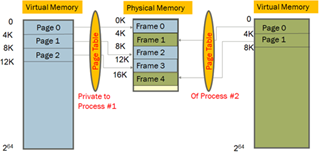
\includegraphics[width=8cm, height=4cm]{313Quiz2P5}
\end{center}

Since the physical memory has no more space for new pages, when process 2 tries to allocate and use another page, a page fault will occur. This means that one of the frames that process 2 is using must be kicked out. If we use LRU caching and assume that page 0 was the least recently used page, we would evacuate page 0 (frame 1) back to the disk and load the new page (page 2) into the newly evacuated spot. Now the page table will map page 0 to the disk and page 2 to frame 1. 

{\bf 6.} [25 pts] Draw the Descriptor Table (DT) and the File Table (FT) for each possible process just after executing the lines 2, 5 and 10 and explain what you see in the standard output and {\bf file.txt} along the way. 

\begin{center}
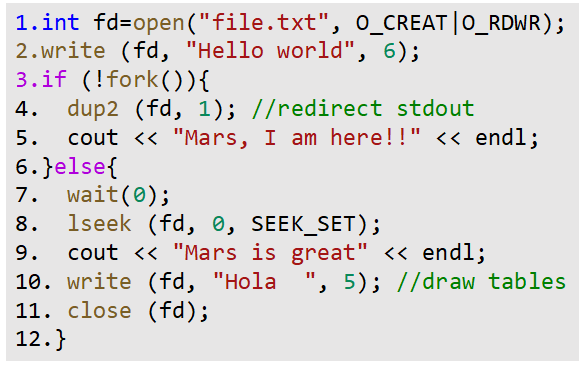
\includegraphics[width=9cm, height=6cm]{P6}
\end{center}

At line 2, fd will take the value of 3 and the file position of file.txt will be 6 since line 2 writes "Hello " and stdout would show nothing. The file-table and descriptor table is shown below. 

\begin{center}
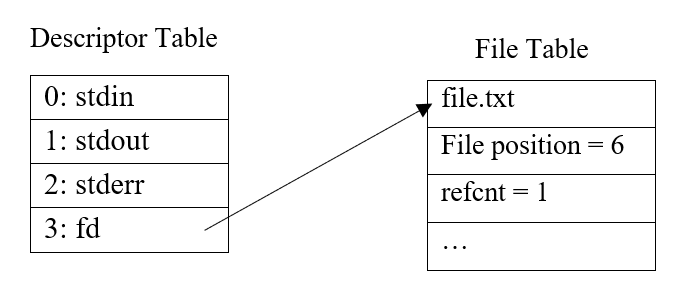
\includegraphics[width=8cm, height=4cm]{P6Line2}
\end{center}

At line 5, a child and parent process has been created due to the fork function call. Within the child process, the stdout file descriptor will point to file.txt. After the call for line 5, file.txt will have "Hello Mars, I am here!!" as its contents as the stdout has been redirected. 

\begin{center}
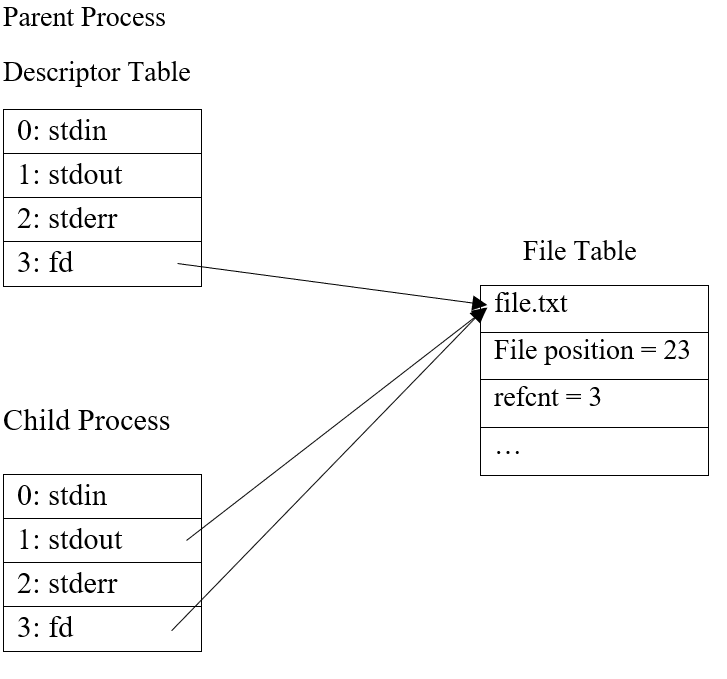
\includegraphics[width=8cm, height=8cm]{P6Line5}
\end{center}

At line 10, no redirection is done with stdout, so the cout statement would print to the terminal. Line 8 changes the file position to the beginning of the file. The standard output would show "Mars is great" and line 10 would overwrite the first 5 characters of file.txt. file.txt would show "Hola  Mars is great" (2 spaces after Hola). 

\begin{center}
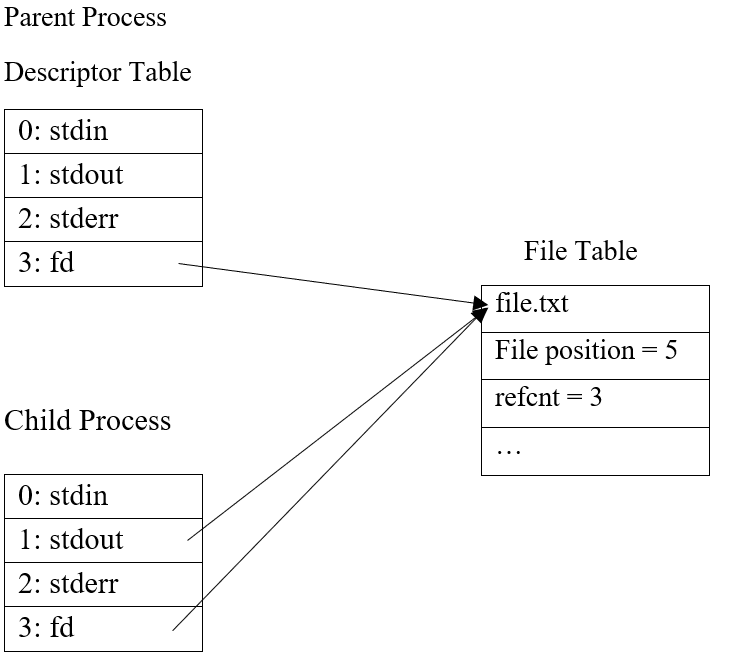
\includegraphics[width=8cm, height=8cm]{P6Line10}
\end{center}

{\bf 7.} [25 pts] Please explain the output of the following program using a process tree diagram as shown in Lecture 4 page 23. Assuming the main process's ID is 1000, explain the order of process creation (in fact, the number itself should show what order the processes are created). Also explain what you see in the standard output. Are different outputs possible for this program? Why or why not? 

\noindent
{\color{violet} for} ({\color{blue} int} i={\color{Green}0}; i$<${\color{Green}4}; i++) \{\\
\tab{\color{blue}int} cid = {\color{RawSienna}fork}();\\
\tab{\color{violet}if}(i$<${\color{Green}2})\\
\tab\tab{\color{RawSienna}wait}({\color{Green}0});\\
\tab cout $<<$ {\color{Maroon}"ID="} $<<$ {\color{RawSienna}getpid}() $<<$ endl;\\
\}

\begin{center}
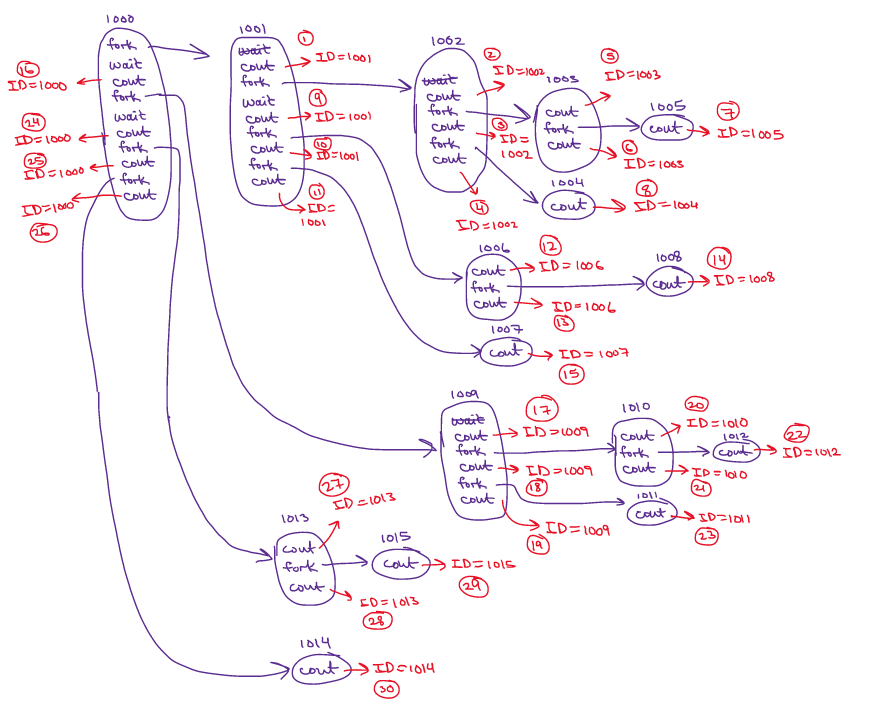
\includegraphics[width=12cm, height=12cm]{P7}
\end{center}

The tree-diagram above shows the order of creation of processes. The items in red show the order in which the print statements occur. The first two forks in process 1000, since wait was called, the parent waited for the child processes to finish before continuing running the rest of its code. After the first two forks, the last two forks didn't wait and simply ran their code before running the child process code. This can be seen through the first two forks as the process ids are incremented in a Depth-First Search manner while the last two forks incremented the process ids in a Breadth-First Search manner. 

The output from this program could vary due to a multitude of reasons. First, the scheduler algorithm could vary leading to different memory allocation which will give different process ids. Also, different systems and different system states could cause different reactions to fork calls. If no wait is present, then either the parent or the child could run first and this is determined at runtime making the output non-deterministic. For this problem, it was assumed that when no wait is called, the parent runs first, then the child. 

\end{document}